\documentclass[a4paper,10pt]{article}
\usepackage[utf8]{inputenc}
\usepackage[french]{babel}
\usepackage{graphicx}
\usepackage{multicol}
\graphicspath{{./img/}}
\usepackage[left=3cm,right=3cm,top=2.5cm,bottom=2cm]{geometry}
\usepackage{url}
\usepackage{subcaption}

\usepackage{fancyhdr}
\pagestyle{fancy}
\fancyhead[L]{Projet S6}
\fancyhead[R]{Rapport de Génération Procédurale}

\fancyfoot[L]{Groupe 12820}
\fancyfoot[R]{Année 2020-2021}
\renewcommand\footrulewidth{0.5pt}

\usepackage{amsmath, amssymb}
\usepackage{tikz}
\usetikzlibrary{arrows,automata,shapes}

\begin{document}
\begin{figure}[h]
    \centering
    
\includegraphics[scale=0.7]{enseirb.png}
\end{figure}
\begin{center}
\Large Rapport de projet - Semestre  - Groupe 12820 \\
\vspace{0.5cm}
Mai 2021
\vspace{2cm}
\begin{figure}[h]
\begin{tikzpicture}[scale=1.3]
\draw (0,0) -- (12,0);  
\end{tikzpicture}
\end{figure}\\
\vspace{1cm}
\textbf{\Huge Génération Procédurale}
\vspace{1cm}
\begin{figure}[h]
\begin{tikzpicture}[scale=1.3]
\draw (0,0) -- (12,0);  
\end{tikzpicture}
\end{figure}\\
\vspace{0.5cm}
Filière Informatique - ENSEIRB-MATMECA
\end{center}
\begin{flushleft}
Auteurs: \\
M.DUCOS Mathieu\\
M.MICHEL Theo\\
M.OUALI Mohammed \\
M.KASOUR Mahmoud\\
\vspace{0.5cm}
Encadrants:\\
M.ROLLET Antoine  \\
M.RENAULT David\\
\end{flushleft}

\newpage
\tableofcontents
\newpage
\section{Introduction}


\subsection{Problématique}
\subsection{Adaptation des concepts de programmation fonctionnelle aux images}
Une image est généralement une matrice de pixels ce qui lui donne un poids de 
8 * 4 * nombre de pixels. Ceci est nécessaire pour les photographies par exemple, celles-ci étant imprévisibles et variées, trouver une fonction qui les représente est très difficile.
Notre objectif étant de représenter des images à l'aide de fonctions, nous allons voir ce que cela implique.
Nous allons ainsi explorer deux extrêmes de la génération procédurale, la génération de bruit, et la génération de motifs réguliers. Ce qui nous permettra ensuite en théorie de les composer pour arriver à n'importe quel résultat entre les deux.

\subsection{Outils de travail}

Afin de pouvoir travailler en équipe et de se partager le code  écrit par chacun. Nous avons utilisé git. Cet outil nous permet par ailleurs en cas de problème avec la dernière version de revenir à la précédente. Ce rapport est lui écrit en \LaTeX , et les fichiers évoqués dans ce rapport sont présents sur le dépôt.






\subsection{Les générateurs}
Le but d'un générateur est de créer des images à partir de diverses règles mathématiques, l'approche naïve est par la programmation impérative, le défi ici a donc été de ne pas céder à la tentation et d'appliquer les principes de la programmation fonctionnelle dans notre projet. Il a donc fallu repenser notre façon de revoir les images, non plus comme un ensemble de pixels, mais plutôt comme une fonction associant à chaque position une valeur (parfois des booléens, parfois une valeur numérique).

\section{Manipulation d'images en programmation fonctionnelle}
La manipulation de l'image est l'endroit ou nous avons du faire une concession par rapport aux précepts de la programmation fonctionnelle, en effet pour modifier tous les pixels d'une image il n'est d'autres choix que de parcourir tous les pixels, ce n'est qu'ensuite que nous avons eu l'occasion d'utiliser les nouveau outils fonctionnels.
\\
L'application des fonctions se fait donc de la manière suivante:
\begin{figure}[h]
    \centering
    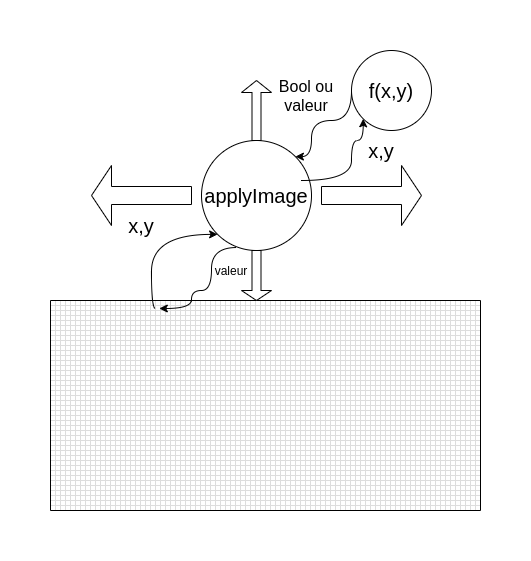
\includegraphics[scale=0.4]{f_forward.png}
    \caption{Méthode d'application des fonctions aux images}
\end{figure}

\newpage

\section{Textures basées sur les calculs de distance}
\subsection{Diagrammes de Voronoi}
Diagramme de Voronoi est un découpage du plan ou dans le sujet pavage en cellules à partir d'un ensemble discret de points qui se trouve aléatoirement sur le pavage appelés « germes ». Chaque cellule renferme un seul germe, et forme l'ensemble des points du plan plus proches de ce germe que de tous les autres. La cellule représente en quelque sorte la « zone d'influence » du germe.\\
\begin{figure}[h]
    \centering
    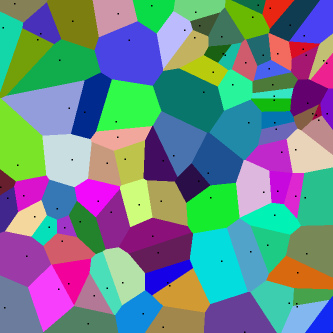
\includegraphics[scale=0.5]{Coloured_Voronoi_2D.png}
\end{figure}\\
Dans le plan on place aléatoirement n points appelés sites ou  germes , chaque germe on l'attribue une couleur aussi aléatoire ,pour créer les cellules on se base sur le fait que la frontière entre les cellules de Voronoi de deux germes distincts se situe forcément sur la médiatrice qui sépare ces deux germes. En effet, les points de cette médiatrice sont équidistants des deux germes donc on ne peut pas affirmer qu’ils se situent dans l'une ou l'autre cellule de Voronoi. Pour un ensemble de germes, le diagramme de Voronoi se construit donc en déterminant les médiatrices de chaque couple de germes. Un point d'une médiatrice appartient alors à une frontière de Voronoi s'il est équidistant d'au moins deux germes et qu'il n'existe pas de distance plus faible entre ce point et un autre germe de l'ensemble. 
on a utilisé dans le cadre de programmation fonctionnel des fonctions déjà implémentés 
comme \texttt{initCanvas} pour initialiser le canvas et \texttt{fillPixel} qui color le pixel et enfin \texttt{Show} pour afficher l'image .
La figure \ref{pseudocodeVor} ci-dessous représente un Pseudo-code pour créer le diagramme de Voronoi :
\vspace{0cm}\\
\begin{ttfamily}
\indent Voronoi \\
\indent debut\\
\indent\indent \textcolor{blue}{Génération des germes aléatoirement }\\
\indent\indent \textcolor{blue}{initCanvas }\\
\indent\indent pour x de 0 a height  faire \\
\indent\indent\indent pour y de 0 a width  faire \\
\indent\indent \indent \textcolor{blue}{fillPixel(x ,y ,couleur de germe ,image)}\\
\indent\indent \textcolor{blue}{displayImage} \\
\indent fin
\end{ttfamily}
\begin{figure}[h]
\caption{Pseudo-code de Voronoi}
\label{pseudocodeVor}
\end{figure}\\
La complexité de cet algorithme est O(n*n) car c'est un algorithme incrémental et il traite les points un par un .
\subsubsection{Voronoi Normale}
En utilisant l'algorithme de Voronoi mais avec des couleurs bien choisis :
une bibliothèque de couleurs a été bien définis pour produire un pavages bien plus assorti 

\begin{figure}[h]
    \centering
    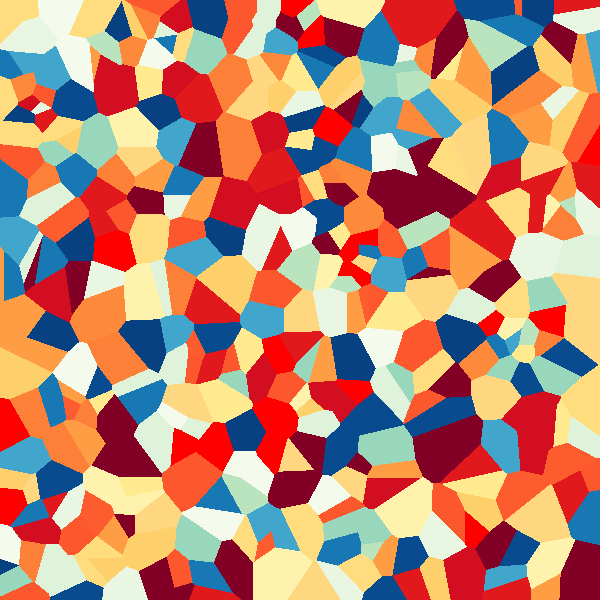
\includegraphics[scale=0.3]{Vor.png}
    \caption{Diagramme de Voronoi}
\end{figure}

\subsubsection{Black Voronoi}
De la même manière et le même algorithme de Voronoi mais en utilisant juste les nuances de la couleur noir on peut générer un beau diagramme de Voronoi  
\begin{figure}[h]
    \centering
    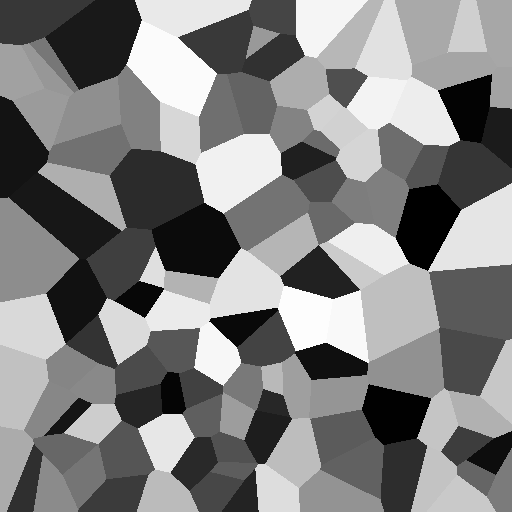
\includegraphics[scale=0.4]{vosBlack.png}
    \caption{Diagramme de Voronoi noir}
\end{figure}


\section{Textures basées sur la génération de bruit spatial}
\subsection{ Bruit de Perlin}
Le bruit de Perlin est une texture procédurale utilisée comme effet visuel pour augmenter le réalisme apparent dans la synthèse d'image .L'algorithme permet de générer procéduralement des textures par bruit de dégradé .
La méthode de génération est la suivante :\\
Nous avons une grille de dimension 2. À chaque coordonnée de la grille, on stocke un vecteur. Pour chaque coordonnée de la matrice, on calcule les produits scalaires de la distance correspondante et celle des vecteurs de dégradé. Puis on interpole ces produits scalaires en utilisant une fonction dont la dérivée primitive et éventuellement dérivée seconde est nulle au niveau des deux points d'extrémité.\\

\begin{figure}[h]
    \centering
    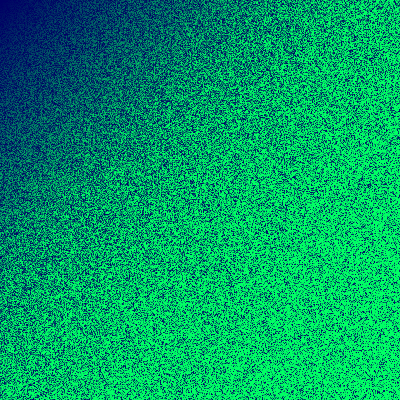
\includegraphics[scale=0.5]{noise.png}
    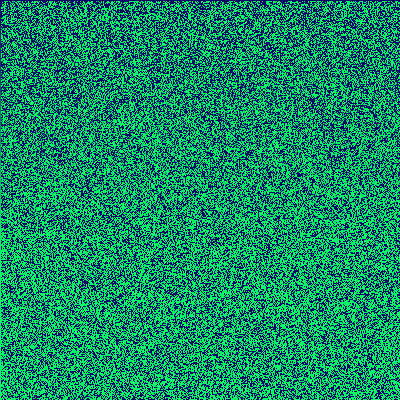
\includegraphics[scale=0.5]{noise1.png}
    \caption{Pavage de Perlin}
\end{figure}


\subsection{ Bruit de Worley }
L'idée de base est de prendre des points aléatoires dans l'espace de 2 dimensions, puis pour chaque emplacement dans l'espace, prendre les distances \texttt{dn} au point le plus proche et utilisez des combinaisons de ceux-ci pour contrôler les informations de couleur par exemple 255 -\texttt{k}*\texttt{dn} et 0 si elle est négative , \texttt{k} contrôle la densité dans le pavage \\
\begin{figure}[h]
\centering
  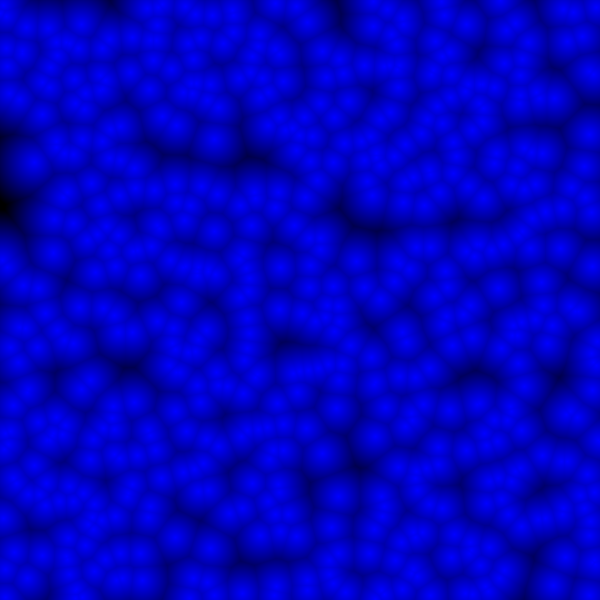
\includegraphics[scale=0.2]{voronoi2.png}
  \caption{Pavages avec bruit de Worley}
  \label{fig1}
\end{figure}
\begin{figure}[h]
\centering
  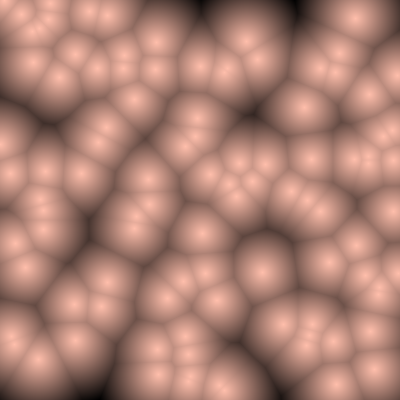
\includegraphics[scale=0.3]{voronoi3.png}
  \caption{Pavages avec bruit de Worley plus dense}
\end{figure}
\\


\section{ Les textures basées sur les pavages}
Après avoir abordé le désordre de la génération de bruits, il convient de revenir en terres plus sereines et d'aborder les pavages.

Les pavages de plans ne sont pas tout le temps possible, en effet il y a plusieurs contraintes géométriques à respecter. Il existe 11 pavages du plan de polygones réguliers. Huit sont des pavages semi-réguliers ,trois sont des pavages réguliers  \\

Dans le cadre de ce projet, il y a une autre contrainte qui se rajoute :
trouver l'algorithme le plus générique possible qui permet de générer tous les pavages.L'utilisateur pouvant l'utiliser en spécialisant ses arguments.\\

L'idée est simple, on part du principe que la propriété géométrique commune à tous les polygones réguliers est l'invariance de la distance entre le barycentre et tous les sommets. Alors on caractérise chaque pavage par le nombre de sommet et cette distance que l'on appelle ("size" dans le code source). \\
Ensuite , on utilise la fonction \textit{PolyFactory(number\_of\_vertex, radius)}, qui renvoie un tableau des positions des sommet du polygone. Cette fonction va être utilisée par la suite pour vérifier si un pixel doit être colorier par une telle couleur en respectant les conditions du pavages obtenues par les fonctions \textit{squareTilingConditon}, \textit{triangleTilingConditon}, \textit{hexTilingCondition}, etc.. \\

Enfin la fonction \textit{applyImage} va prendre en paramètre autant de conditions que de couleurs, parcourant tous les pixels et en fonction de la valeur retournée par  \textit{Sumfunctions} , décide par quelle couleur on va le colorier .
\\
Voir les commentaires du code pour plus de détailles.
La complexité de la fonction applyImage est $O(\frac{s*n**(5/2}{size})$  s étant égale au nombre de sommet de chaque polygone et size la distance du barycentre au centre.
\\
Cette méthode permet de générer des pavages avec des polygones réguliers en spécialisant ses paramètres d'entrée. L'utilisateur doit créer les fonctions de type \textit{ConditionForSquareTiling} qui correspondent au pavage qu'il souhaite réaliser si il veut être précis, utilisant la fonction générique polygoneDrawingPattern\\
Pour montrer la généricité de notre code nous avons également créé une interface web.
\subsection{Interface Web}

\begin{figure}[h]
    \centering
    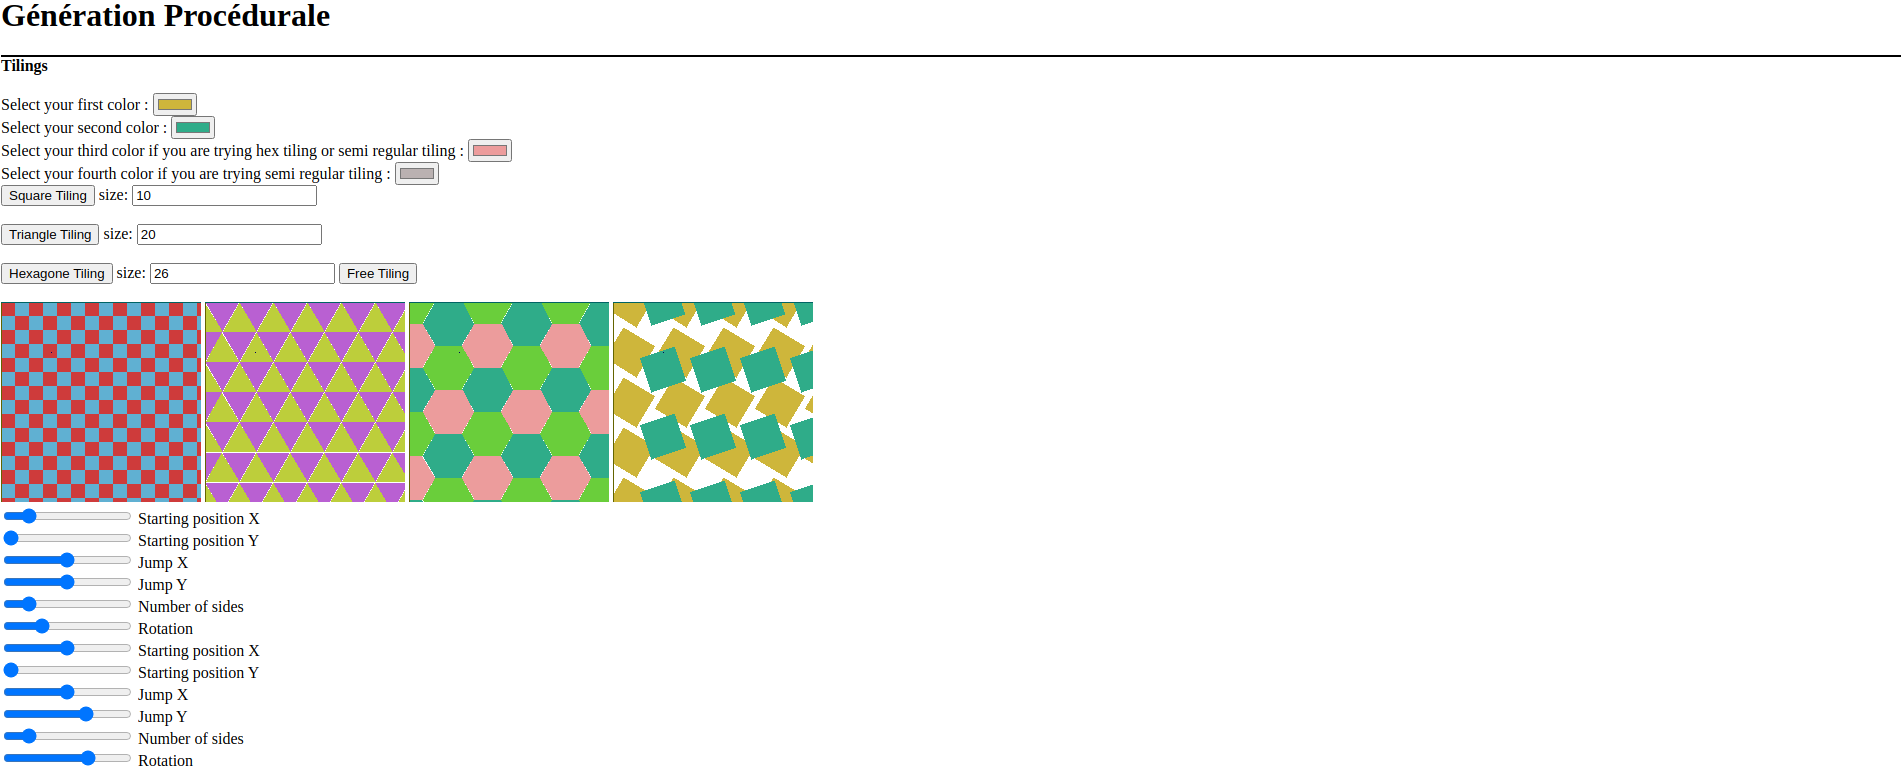
\includegraphics[scale=0.5]{web_interface.png}
    \caption{Interface Web}
\end{figure}
Pour utiliser l'interface il faut faire
make \\
puis node dist/index.html
On peut voir grâce aux sliders sur le bas de la page que les pavages sont hautement personalisable dans tous les sens.




\section{Améliorations envisageables}
\subsection{Solutions algorithmiques moins complexes}
la complexité d'algorithme de Voronoi est O(n*n) mais en utilisant l'algorithme de Fortune on peut aboutir à une complexité en O(n*log n) l'idée c'est de construire le diagramme de Voronoï progressivement en balayant le plan de gauche à droite avec une ligne verticale .


\section{Filtres réalisé}
\subsection{filtres réalisant la composition de deux images}
Afin de réaliser la composition de deux images nous avons implémenté une fonction \texttt{printOperation} celle ci prend 2 images en entrée et retourne en sortie une image étant la composition de ces deux images, les fonctions que nous avons implémenté sont le produit et la division. Pour réaliser cela pour chacun des pixels nous avons fait le produit des deux pixels. Ainsi on obtient dans le cas su produit une image qui noircit alors que dans le cas du screen au contraire l'image va s'éclaircir. Exemple de composition d'image:\\

\begin{figure}[ht]
     \centering
     \begin{subfigure}[b]{.25\textwidth}
         \centering
         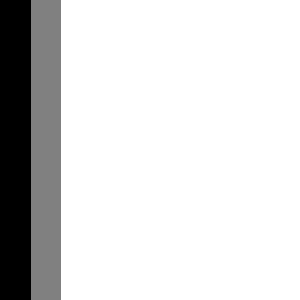
\includegraphics[scale=0.3]{whitheBlackH.png}
         \caption{image avec des bandes horizontale }


     \end{subfigure}
     \hfill
     \begin{subfigure}[b]{0.25\textwidth}
         \centering
         
\includegraphics[scale=0.3]{whitheBlackV.png}
        \caption{image avec des bandes horizontale }
     \end{subfigure}
     \hfill
     \centering
     \begin{subfigure}[b]{0.25\textwidth}
         \centering
         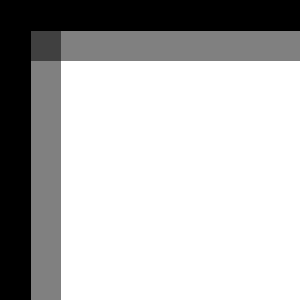
\includegraphics[scale=0.3]{firstProduct.png}
        \caption{produit des deux premières images}
     \end{subfigure}
     \hfill
     \begin{subfigure}[b]{0.5\textwidth}
         \centering
    
\includegraphics[scale=0.3]{firstScreen.png}
            \caption{graphe serpent}
     \end{subfigure}
        \caption{Exemple de compositions d'images}
\end{figure}

Dans le cas de ces compositions cela fonctionne donc bien.
\subsection{Produit de convolution} 
Nous avons aussi essayé de créer des filtres à base de technique de convolution les méthodes ont été implémentée cependant les tests que nous avons fait nous montre que les résultats obtenues ne sont pas exactement ce qu'il devrait être. 
\begin{figure}[h]
\centering
  
\includegraphics[scale=0.5]{convol1.png}
  \caption{Filtres avec méthode de convolution dessinant les contours d'une image}
\end{figure}
\\
Pour réaliser cette figure nous avons utilisé la fonction \texttt{applyFilter} celle ci modifie l'image en fonction du produit de convolution choisi. On parcours alors tous les pixels et pour chaque pixel on réalise le produit de convolution de la matrice composé de ce pixel et de ses voisins soit en formant une image composé de 9 ou de 25 pixels. On obtient alors une valeur qui devient ce la nouvelle coloration du pixel.

\section{Conclusion}
Ce projet a permis à la plupart des membres du groupe d'acquérir de nouvelles compétences. Cela nous a aussi permis de comprendre mieux certaines parties du cour particulièrement en js mais aussi dans la maîtrise d'eslint et des interfaces html.
\newline

Nous avons apprécier de pouvoir travailler sur les projets en présentiel c'est pour nous un vrai plus par rapport au premier semestre ou nous n'avions pas forcément toujours vu nos camarades. De plus pour demander de l'aide que ce soit aux enseignant ou à d'autres élèves cela aide beaucoup.
\newline

Nous avons cependant eu beaucoup de mal à atteindre les objectifs de ce projet; comme nous avons tous été en difficulté au premier semestre nous avions des rattrapages à travailler pendant les premières semaines de projet ce qui ne nous a pas aidé à nous concentrer dessus à leur début
\newline

Nous tenions à remercier notre encadrant  Monsieur Antoine ROLLET, ainsi que notre responsable de projet Monsieur David Renault pour l'aide qu'ils nous ont apporté tout au long de ce projet.




\section{Références}

https ://www.labri.fr/perso/renault/working/teaching/projets/
\\
\indent https ://thor.enseirb-matmeca.fr/
\\
\indent https://www.labri.fr/perso/renault/working/teaching/projets/ladder/ladder.html
\\
\indent https://www.gnu.org/software/gsl/
\\




\end{document}